% +------------------------------------------------------------------------+
% | CGAL Reference Manual:  polyhedron.tex
% +------------------------------------------------------------------------+
% | Combinatoric and geometry of polyhedral surfaces in 
% | halfedge representation.
% |
% | 11.10.1996   Lutz Kettner
% |              Start rewriting the whole stuff
% | 
\RCSdef{\polyhedronRev}{$Revision$}
\RCSdefDate{\polyhedronDate}{$Date$}
% +------------------------------------------------------------------------+

\ccParDims

\chapter{3D-Polyhedral Surfaces}
\label{chapterPolyhedron}
\ccChapterRelease{\polyhedronRev. \ \polyhedronDate}\\
\ccChapterAuthor{Lutz Kettner}


% +------------------------------------------------------------------------+
\section{Introduction}
\label{sectionPolyIntro}

Polyhedral surfaces in three dimensions are composed of vertices,
edges, facets and an incidence relationship on them. The organization
beneath is a halfedge data structure, which restricts the class of
representable surfaces to orientable 2-manifolds -- with and without
boundary. If the surface is closed we call it a {\em polyhedron}, for
example the following model of a hammerhead:

\begin{ccTexOnly}
    \vspace*{-4mm}
    \begin{center}~\hspace{1cm}
      \parbox{0.55\textwidth}{%
          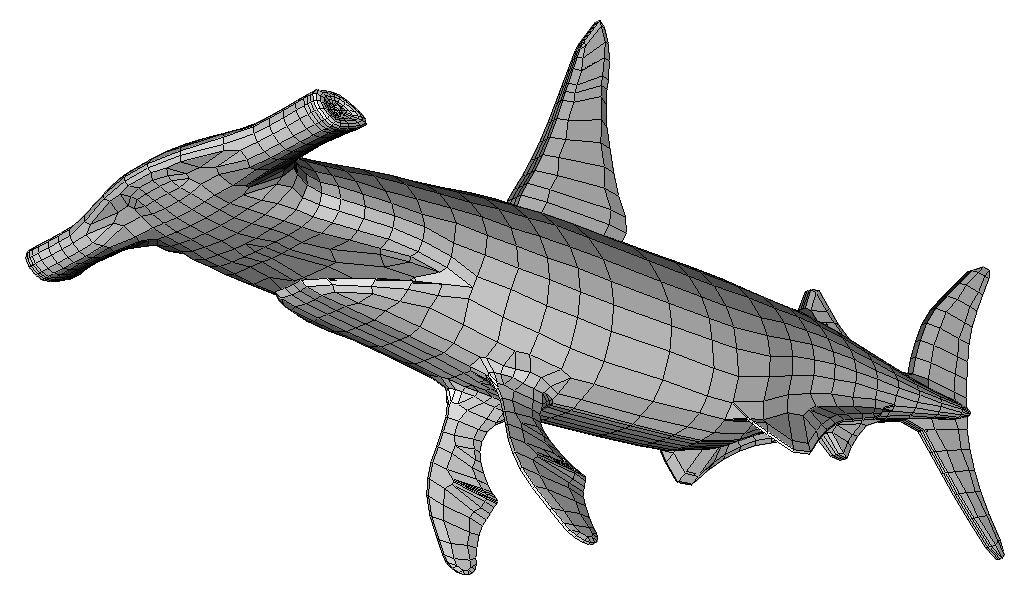
\includegraphics[width=0.55\textwidth]{fig/shark.ps}%
      }
    \end{center}
    \vspace*{-4mm}
\end{ccTexOnly}

\begin{ccHtmlOnly}
    <CENTER>
        <img src="./shark.gif" alt="Hammerhead"><P>
    </CENTER>
\end{ccHtmlOnly}

The polyhedral surface is realized as a container class that manages
vertices, halfedges, facets with their incidences, and that maintains
the combinatorial integrity of them. It is based on the highly
flexible design of the halfedge data structure, see the introduction
in Chapter~\ref{chapterHalfedgeDS} and~\cite{k-ugpdd-99}, but the
following examples can be understood without knowing the underlying
design.

% +========================================================================+
\section{Definition}
% +========================================================================+
  
A polyhedral surface \ccc{CGAL::Polyhedron_3<Traits>} in three dimensions
consists of vertices $V$, edges $E$, facets $F$ and an incidence
relation on them.  Each edge is represented by two halfedges with
opposite orientations. The incidences stored with a halfedge are
illustrated in the following figure:

\begin{ccTexOnly}
    \vspace{-7mm}
    \begin{center}
      \parbox{0.4\textwidth}{%
          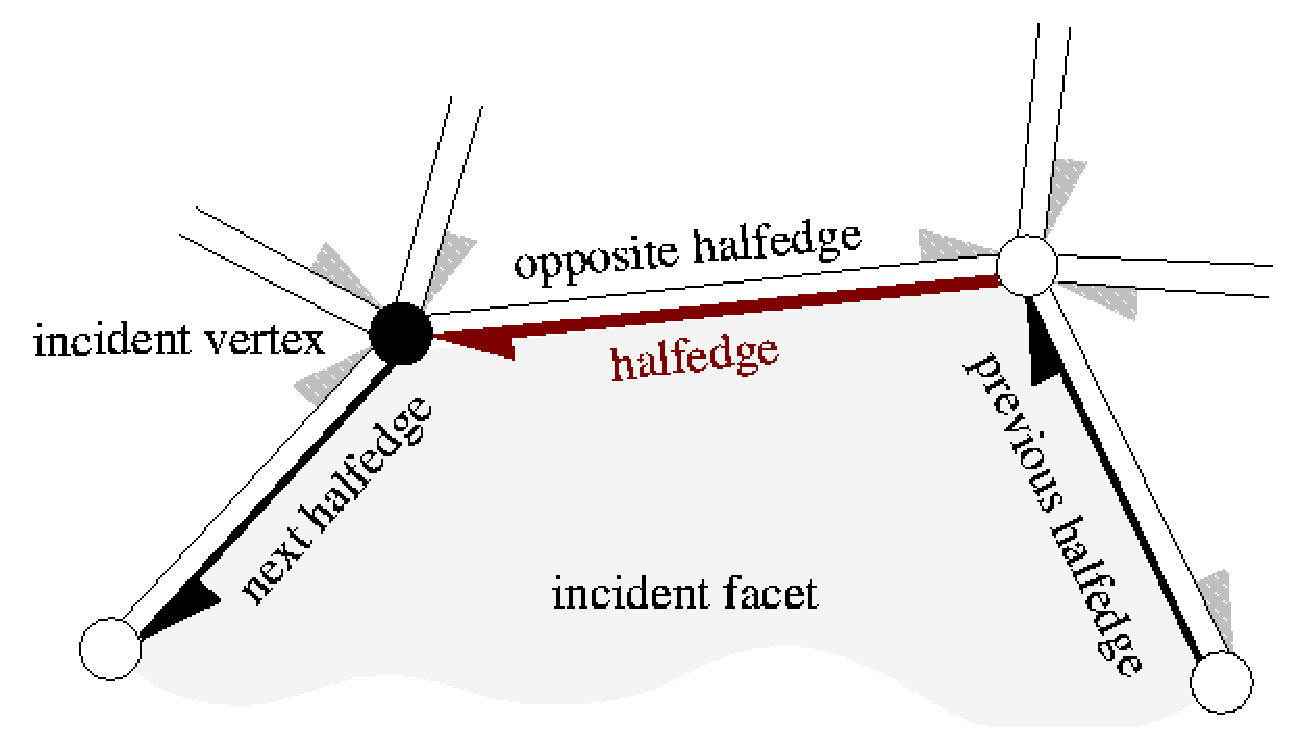
\includegraphics[width=0.4\textwidth]{fig/halfedge.ips}%
      }
    \end{center}
    \vspace{-5mm}
\end{ccTexOnly}

\begin{ccHtmlOnly}
    <CENTER>
    <A HREF="./halfedge.gif">
        <img src="./halfedge_small.gif" alt="Halfedge Diagram"></A><P>
    </CENTER>
\end{ccHtmlOnly}

Vertices represent points in space. Edges are straight line segments
between two endpoints. Facets are planar polygons without
holes. Facets are defined by the circular sequence of halfedges along
their boundary.  The polyhedral surface itself can have holes (with at
least two facets surrounding it since a single facet cannot have a
hole). The halfedges along the boundary of a hole are called {\em
border halfedges\/} and have no incident facet. An edge is a {\em
border edge\/} if one of its halfedges is a border halfedge.  A
surface is {\em closed\/} if it contains no border halfedges. A closed
surface is a boundary representation for polyhedra in three
dimensions. The convention is that the halfedges are oriented
counterclockwise around facets as seen from the outside of the
polyhedron. An implication is that the halfedges are oriented
clockwise around the vertices. The notion of the solid side of a facet
as defined by the halfedge orientation extends to polyhedral surfaces
with border edges although they do not define a closed object. If
normal vectors are considered for the facets, normals point outwards
(following the right-hand rule).

The strict definition can be found in~\cite{k-ugpdd-99}. One
implication of this definition is that the polyhedral surface is
always an orientable and oriented 2-manifold with border edges, i.e.
the neighborhood of each point on the polyhedral surface is either
homeomorphic to a disc or to a half disc, except for vertices where
many holes and surfaces can join. Another implication is that the
smallest representable surface avoiding self intersections is a
triangle (for polyhedral surfaces with border edges) or a tetrahedron
(for polyhedra). Boundary representations of orientable 2-manifolds
are closed under Euler operations. They are extended with operations
that create or close holes in the surface.

Other intersections besides the incidence relation are not allowed.
However, this is not automatically verified in the operations, since
self intersections are not easy to check
efficiently. \ccc{CGAL::Polyhedron_3<Traits>} does only maintain the
combinatorial integrity of the polyhedral surface (using Euler
operations) and does not consider the coordinates of the points or any
other geometric information.

\ccc{CGAL::Polyhedron_3<Traits>} can represent polyhedral surfaces as
well as polyhedra. The interface is designed in such a way that it is
easy to ignore border edges and work only with polyhedra.


% +========================================================================+
\section{Example Programs}
% +========================================================================+
\label{sectionPolyExamples}

The polyhedral surface is based on the highly flexible design of the
halfedge data structure. Examples for this flexibility can be found in
Section~\ref{sectionPolyExtend} and in Section~\ref{sectionHdsExamples}. 
This design is not a prerequisite to understand the following examples.
See also the Section~\ref{sectionPolyAdvanced} below for some advanced 
examples.

% +-------------------------------------------------------------+
\subsection{First Example Using Defaults}

The first example instantiates a polyhedron using the default traits
class. It creates a tetrahedron.

\newpage
\ccIncludeExampleCode{Polyhedron/polyhedron_prog_simple.C}

% +-------------------------------------------------------------+
\subsection{Example with Geometry in Vertices}

This example creates a tetrahedron initialized with four points. In
addition it demonstrates the use of the vertex iterator and the access
to the point in the vertices. The output of
the program will be ``\verb|1 0 0\n0 1 0\n0 0 1\n0 0 0\n|''.

\ccIncludeExampleCode{Polyhedron/polyhedron_prog_tetra.C}

The polyhedron offers a point iterator for convenience. The above
output simplifies to a single statement by using the \stl\ algorithm
\ccc{std::copy} and the ostream iterator adaptor.

\begin{ccExampleCode}
std::copy( P.points_begin(), P.points_end(), 
           std::ostream_iterator<Point>(std::cout,"\n"));
\end{ccExampleCode}

% +-------------------------------------------------------------+
\subsection{Example for Affine Transformation}

Assuming that only the point coordinates of a polyhedron $P$ need to
be transformed by an affine transformation $A$, the \stl\ algorithm
\ccc{std::transform} can be used. 

\begin{ccExampleCode}
std::transform( P.points_begin(), P.points_end(), P.points_begin(), A);
\end{ccExampleCode}

The point iterator is already conveniently defined for polyhedral
surfaces. However, for other geometric attributes, such iterators
need to be defined by the user. This can be done easily, see the
following example about adding a plane equation for facets.


% +-------------------------------------------------------------+
\subsection{Example Computing Plane Equations}

The polyhedral surface has already provisions to store a plane
equation---or only its normal vector---for each facet. However, it 
does not have a function to compute plane equations or normal vectors. 

This example computes the plane equations for the facets of a
tetrahedron.  The actual plane computation is provided in the user
defined function {\tt compute\_plane\_equations}.  Depending on the
coordinate number type (exact/inexact) and the shape of the polygons
of facets (convex/non-convex) different methods are possible. We
assume here strictly convex facets and exact arithmetic. In our
example a homogeneous representation with {\tt int} coordinates is
sufficient.  The output of the program are the four plane
equations. 

For the output, we define a \texttt{Plane\_iterator} similar to the point
iterator already provided by the polyhedron class. We use the
\texttt{CBP\_Project\_iterator} from the support library. It takes a projector 
function object, \texttt{CBP\_Project\_plane}, that given a reference
to a facet returns a reference to its plane equation. Here is the
implementation of this projector. Others can be written easily.

\begin{ccExampleCode}
template < class Facet>
struct Project_plane {
    typedef Facet                  argument_type;
    typedef typename Facet::Plane  Plane;
    typedef Plane                  result_type;
    Plane&       operator()( Facet& x)       const { return x.plane(); }
    const Plane& operator()( const Facet& x) const { return x.plane(); }
};
\end{ccExampleCode}

Note that in distinction to normal function objects we work here with
references and have a second member function for the const-references
version of this call. The example for computing the plane equations
follow.

\ccIncludeExampleCode{Polyhedron/polyhedron_prog_normals.C}

% +-------------------------------------------------------------+
\subsection{Example with a Vector instead of a List Representation}
\label{sectionPolyVector}

The polyhedron class template has actually three parameters, where two
of them have default values. Using the default values explicitly in
our examples above, the definition of a polyhedron looks like:

\begin{ccExampleCode}
typedef CGAL::Polyhedron_3< Traits, 
                            CGAL::Polyhedron_items_3, 
                            CGAL::HalfedgeDS_default>      Polyhedron;
\end{ccExampleCode}

The \ccc{CGAL::Polyhedron_items_3} class contains the types used for
vertices, edges and facets. The \ccc{CGAL::HalfedgeDS_default} class
defines the halfedge data structure used, which is a list-based
representation in this case. An alternative is a vector-based
representation. Using a vector provides random
access for the elements in the polyhedral surface and is more space
efficient, but elements cannot be deleted arbitrarily. Using a list
allows arbitrary deletions, but provides only bidirectional iterators
and is less space efficient. The following example creates again a 
tetrahedron with given points, but in a vector-based representation.

The vector-based representation resizes automatically if the reserved
capacity is not sufficient for the new items created. Upon resizing
all handles, iterators, and circulators invalidate. Their correct
update in the halfedge data structure is costly, thus it is advisable
to reserve enough space in advance as indicated with the alternative
constructor in the comment. Advanced remark: Note that the polyhedron
and not the underlying halfedge data structure triggers the resize
operation, since the resize operation requires some preconditions,
such as valid incidences, to be fulfilled that only the polyhedron can
guarantee.

\ccIncludeExampleCode{Polyhedron/polyhedron_prog_vector.C}


% +-------------------------------------------------------------+
\subsection{Example Writing Object File Format (OFF)}

The following example creates a tetrahedron and writes it to
\ccc{std::cout} using the Object File Format (OFF)~\cite{p-gmgv15-94}.  The
example makes use of \stl\ algorithms (\ccc{std::copy}, \ccc{std::distance}),
\stl\ \ccc{std::ostream_iterator}, and \cgal\ circulators.  However, the
computation of the vertex index in the inner loop of the facet output
is not advisable with the \ccc{std::distance} function, since it takes
linear time for non random-access iterators, which results in a
quadratic runtime for the whole output. For better runtime the vertex
index needs to be stored separately and computed once before writing
the facets. It can be stored, for example, in the vertex itself or in
a hash-structure.  See also the following Section~\ref{sectionPolyIO}
on existing support for file I/O in the library.

\ccIncludeExampleCode{Polyhedron/polyhedron_prog_off.C}


% +========================================================================+
\section{File I/O}
% +========================================================================+
\label{sectionPolyIO}

Simple file I/O for polyhedral surfaces is already provided in the
library. The file I/O considers so far only the topology of the
surface and its point coordinates. It ignores a possible plane
equation, normal vector, or any user-added attributes, such as color.

The default file format supported in \cgal\ for output as well as for
input is the Object File Format, OFF, with file extension {\tt .off},
which is also understood by GeomView~\cite{p-gmgv15-94}. For OFF
exists an ASCII and a binary format. The format can be selected with
the \cgal\ modifiers for streams, \ccc{set_ascii_mode} and
\ccc{set_binary_mode} respectively. The modifier \ccc{set_pretty_mode}
can be used to allow for structuring comments in the
output. Otherwise, the output would be free of comments.  The default
for writing is ASCII without comments. Both, ASCII and binary format,
can be read independant of the stream setting. Since this file format
is the default format, iostream operators are provided for it.

\ccThree{Inventor_ostream&M}{}{.}
\ccInclude{CGAL/IO/Polyhedron_iostream.h}

\ccHtmlNoLinks
\ccGlobalFunction{template <class Traits>
    ostream& operator<<( ostream& out, const CGAL::Polyhedron_3<Traits>& P);}

\ccHtmlNoLinks
\ccGlobalFunction{template <class Traits>
    istream& operator>>( istream& in, CGAL::Polyhedron_3<Traits>& P);}


Additional formats supported for writing are OpenInventor ({\tt .iv})
\cite{w-impoo-94}, VRML 1.0 and 2.0 ({\tt .wrl})
\cite{bpp-vrml-95,vrmls-96,hw-vrml2h-96}, and Wavefront Advanced
Visualizer object format ({\tt .obj}). Another convenient output
function writes a polyhedral surface to a GeomView process spawned
from the \cgal\ program.  These output functions are provided as
stream operators, now acting on the stream type of the respective
format.

\ccInclude{CGAL/IO/Inventor_ostream.h}
\\
\ccInclude{CGAL/IO/VRML_1_ostream.h}
\\
\ccInclude{CGAL/IO/VRML_2_ostream.h}
\\
\ccInclude{CGAL/IO/Geomview_stream.h}

\ccHtmlNoLinks
\ccGlobalFunction{template <class Traits>
    Inventor_ostream& operator<<( Inventor_ostream& out, 
                                  const CGAL::Polyhedron_3<Traits>& P);}

\ccHtmlNoLinks
\ccGlobalFunction{template <class Traits>
    VRML_1_ostream& operator<<( VRML_1_ostream& out, 
                                  const CGAL::Polyhedron_3<Traits>& P);}

\ccHtmlNoLinks
\ccGlobalFunction{template <class Traits>
    VRML_2_ostream& operator<<( VRML_2_ostream& out, 
                                  const CGAL::Polyhedron_3<Traits>& P);}

\ccHtmlNoLinks
\ccGlobalFunction{template <class Traits>
    Geomview_stream& operator<<( Geomview_stream& out, 
                                  const CGAL::Polyhedron_3<Traits>& P);}


These file formats have all in common that they represent a surface as
a set of facets. Each facet is a list of indices pointing into a set
of vertices. Vertices are represented as a coordinate triples. The
file I/O for polyhedral surfaces
\ccc{CGAL::Polyhedron_3} imposes certain restrictions onto these
formats. They must represent a permissible polyhedral surface, e.g., a
2-manifold and no isolated vertices, see Section~\ref{sectionPolyIntro}.

Some example programs around the different file formats are provided
in the distribution under \texttt{examples/Polyhedron\_IO/} and
\texttt{demo/Polyhedron\_IO/}.


% +========================================================================+
\section{Extending Vertices, Halfedges, and Facets}
% +========================================================================+
\label{sectionPolyExtend}

In Section~\ref{sectionPolyVector} we have seen how to change the 
default list representation

\begin{ccExampleCode}
typedef CGAL::Polyhedron_3< Traits, 
                            CGAL::Polyhedron_items_3, 
                            CGAL::HalfedgeDS_default>      Polyhedron;
\end{ccExampleCode}

to a vector based representation of the underlying halfedge data
structure. Now we want to look a bit closer at the second template argument,
\texttt{CBP\_Polyhedron\_items\_3}, that specifies what kind of vertex, 
halfedge, and facet is used. The implementation of 
\texttt{CBP\_Polyhedron\_items\_3} looks a bit involved with nested 
wrapper class templates. But ignoring this technicality, what remains
are three local typedefs that define the \texttt{Vertex}, the
\texttt{Halfedge}, and the \texttt{Face} for the polyhedral surface.
Note that we use here \texttt{Face} instead of facet. Face is the term
used for the halfedge data structure. Only the top layer of the
polyhedral surface gives alias names renaming face to facet.

\begin{ccExampleCode}
class Polyhedron_items_3 {
public:
    template < class Refs, class Traits>
    struct Vertex_wrapper {
        typedef typename Traits::Point Point;
        typedef CGAL::HalfedgeDS_vertex_base< Refs, CGAL::Tag_true, Point> Vertex;
    };
    template < class Refs, class Traits>
    struct Halfedge_wrapper {
        typedef CGAL::HalfedgeDS_halfedge_base< Refs> Halfedge;
    };
    template < class Refs, class Traits>
    struct Face_wrapper {
        typedef CGAL::HalfedgeDS_face_base< Refs, CGAL::Tag_true, Traits> Face;
    };
};
\end{ccExampleCode}

If we look up in the reference manual the definitions of the three
classes used in the typedefs, we will see the confirmation that the
default polyhedron uses all supported incidences, a point in the
vertex class, and a plane equation in the face class. Note how the
wrapper class provides two template parameters, \texttt{Refs}, which
we discuss a bit later, and \texttt{Traits}, which is the geometric
traits class used by the polyhedral surface and which provides us here
with the types for the point and the plane equation.

Using this example code we can write our own items class. Instead, we
illustrate an easier way if we only want to exchange one class. We use
a simpler face without the plane equation but with a color attribute
added. To simplify the creation of a vertex, halfedge, or face class,
it is always recommended to derive from one of the given base classes,
even if the base class would contain no data. So, we derive from the
base class, repeat the mandatory constructors if necessary---which is
not the case for faces but would be for vertices---and add the color
attribute.

\begin{ccExampleCode}
template <class Refs>
struct My_face : public CGAL::HalfedgeDS_face_base<Refs> {
    CGAL::Color color;
};
\end{ccExampleCode}

The new items class is derived from the old items class and the
wrapper containing the face typedef gets overridden. Note that the
name of the wrapper and its template parameters are fixed. They cannot
be changed even if, as in this example, a template parameter is not
used.

\begin{ccExampleCode}
struct My_items : public CGAL::Polyhedron_items_3 {
    template <class Refs, class Traits>
    struct Face_wrapper {
        typedef My_face<Refs> Face;
    };
};
\end{ccExampleCode}

When we use our new items class with the polyhedral surface, our new
face class is used in the halfedge data structure and the color
attribute is available in the type \texttt{Polyhedron::Facet}. However,
\texttt{Polyhedron::Facet} is not the same type as our local face 
typedef, but it is derived from the local face typedef. Thus,
everything that we put in the local face type except constructors is then
available in the \texttt{Polyhedron::Facet} type. For more details, see 
the Chapter~\ref{chapterHalfedgeDS} on the halfedge data structure design.

Pulling all together, the full example program illustrates how easy
the color attribute can be accessed once it is defined.

\ccIncludeExampleCode{Polyhedron/polyhedron_prog_color.C}

We come back to the first template parameter, \texttt{Refs}, of the
wrapper classes. This parameter provides us with local types that
allow us to make further references between vertices, halfedges, and
facets, which have not already been prepared for in the current
design. These local types are \texttt{Vertex\_handle},
\texttt{Halfedge\_handle}, \texttt{Face\_handle}, and there respective
\texttt{\ldots\_const\_handle}. We could add now a new vertex reference to a
face class as follows. Encapsulation and access functions could be
added for a more thorough design. The integration of the face class
with the items class works as illustrated above.

\begin{ccExampleCode}
template <class Refs>
struct My_face : public CGAL::HalfedgeDS_face_base<Refs> {
    typedef typename Refs::Vertex_handle Vertex_handle;
    Vertex_handle vertex_ref;
};
\end{ccExampleCode}

More advanced examples can be found in the
Section~\ref{sectionHdsExamples} illustrating the design of the
halfedge data structure.


% +========================================================================+
\section{Advanced Example Programs}
% +========================================================================+
\label{sectionPolyAdvanced}

% +------------------------------------------------------------------------+
\subsection{Example Creating a Subdivision Surface}

This program reads a polyhedral surface from the standard input and
writes a refined polyhedral surface to the standard output. Input and
output are in the Object File Format, OFF, with the common file
extension {\tt .off}, which is also understood by
GeomView~\cite{p-gmgv15-94}.

The refinement is a single step of the $\sqrt{3}$-scheme for creating
a subdivision surface~\ref{k-s-00}. Such a single step subdivides
each facet into triangles around a new center vertex, smoothes the
position of the old vertices, and flips the old edges. The program is
organized along this outline. In each of these parts, the program
efficiently uses the knowledge that the newly created vertices, edges,
and facets have been added to the end of the sequences. The program
needs additional processing memory only for the smoothing step of the
old vertices.

The following figure shows an example of five consecutive subdivision
steps starting with a cube as the initial polyhedral surface.

\begin{ccTexOnly}
    \begin{center}
      \parbox{\textwidth}{%
          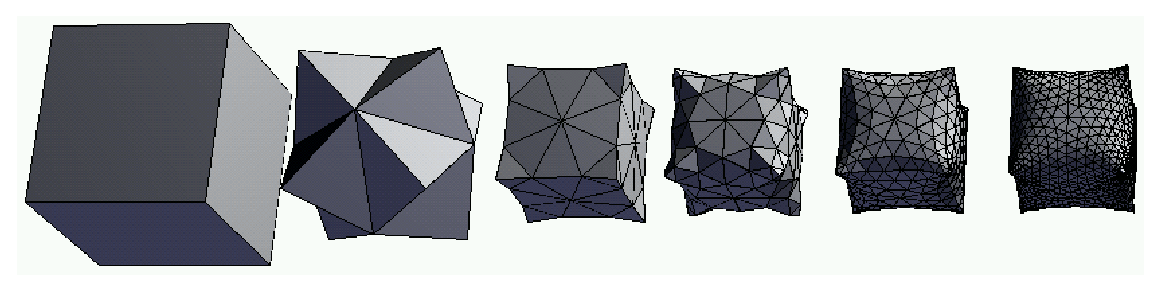
\includegraphics[width=\textwidth]{fig/cube_subdiv.ps}%
      }
    \end{center}
\end{ccTexOnly}

\begin{ccHtmlOnly}
    <CENTER>
        <img src="./cube_subdiv.gif" 
          alt="five consecutive subdivision steps starting with a cube"><P>
    </CENTER>
\end{ccHtmlOnly}

\ccIncludeExampleCode{Polyhedron/polyhedron_prog_subdiv.C}

% +------------------------------------------------------------------------+
\subsection{Example Using the Incremental Builder and Modifier Mechanism}

\begin{ccAdvanced}

A utility class \ccc{CGAL::Polyhedron_incremental_builder_3} helps in
creating polyhedral surfaces from a list of points followed by a list
of facets that are represented as indices into the point list. This is
particularly useful in combination with common file formats for
polyhedra.  It is used here to create a triangle.

A modifier mechanism allows to access the internal representation of
the polyhedral surface, i.e.~the halfedge data structure, in a
controlled manner. A modifier is basically a callback mechanism using
a function object. When called, the function object receives the
internal halfedge data structure as a parameter and can modify it.  On
return, the polyhedron can check the halfedge data structure for
validity. Such a modifier object must always return with a halfedge
data structure that is a valid polyhedral surface.

In this example, \ccc{Build_triangle} is such a function object
derived from \ccc{CGAL::Modifier_base<HDS>}. The \ccc{delegate()} member
function of the polyhedron accepts this function object and calls its
\ccc{operator()} with a reference to its internally used halfedge data
structure. Thus, this member function in \ccc{Build_triangle} can
create the triangle in the halfedge data structure.

\ccIncludeExampleCode{Polyhedron/polyhedron_prog_incr_builder.C}

\end{ccAdvanced}

% +--------------------------------------------------------+

% =============================================================================
% The CGAL Reference Manual
% Chapter: Geometric Optimisation
% -----------------------------------------------------------------------------
% file   : doc_tex/basic/Optimisation/Optimisation_ref/main.tex
% package: Optimisation_doc
% author : Sven Sch�nherr <sven@inf.ethz.ch>
% -----------------------------------------------------------------------------
% $Revision$
% $Date$
% =============================================================================

\section{Reference Pages}

% =============================================================================
% The CGAL Reference Manual
% Chapter: Geometric Optimisation
% -----------------------------------------------------------------------------
% file   : doc_tex/basic/Optimisation/Optimisation_ref/reference_part.tex
% package: Optimisation_doc
% author : Sven Sch�nherr <sven@inf.ethz.ch>
% -----------------------------------------------------------------------------
% $Revision$
% $Date$
% =============================================================================

\newcommand{\inputOpt}[1]{\input{Optimisation_ref/#1.tex}}

\newcommand{\linebreakByHand}{\ccTexHtml{\linebreak[4]}{}}
\newcommand{  \newlineByHand}{\ccTexHtml{\\}{}}

% cross references
\index{minimum enclosing|see{{smallest enclosing}}}
\index{minimum spanning|see{{smallest enclosing}}}
\index{concentric spheres|see{{annulus}}}

% -----------------------------------------------------------------------------
\section*{Introduction}

This chapter describes concepts, classes, and functions for solving
geometric optimisation problems. They are divided into four categories.

\paragraph{Bounding Areas and Volumes.}
Smallest enclosing circle and ellipse (2D), smallest enclosing rectangle,
parallelogram, and strip (2D), rectangular $p$-center (2D), smallest
enclosing sphere and annulus (dD).

\paragraph{Inscribed Areas.}
Maximum area and perimeter inscribed $k$-gon (2D), extremal inscribed
$k$-gon (2D).

\paragraph{Optimal Distances.}
All furthest neigbors (2D), width of point set (3D), polytope distance (dD).

\paragraph{Advanced Techniques.}
Monotone and sorted matrix search.

\section*{Assertions}
The optimisation code uses infix \ccc{OPTIMISATION} in the assertions,
e.g.\ defining the compiler flag
\ccc{CGAL_OPTIMISATION_NO_PRECONDITIONS} switches precondition
checking off, cf.~\cgalReferToAssertions


% -----------------------------------------------------------------------------
\subsection*{Bounding Areas and Volumes}

\ccRefIdfierPage{CGAL::Min_circle_2<Traits>}\\[1ex]
\ccRefIdfierPage{CGAL::Min_circle_2_traits_2<K>}\\[1ex]
\ccRefConceptPage{MinCircle2Traits}

\smallskip

\ccRefIdfierPage{CGAL::Min_ellipse_2<Traits>}\\[1ex]
\ccRefIdfierPage{CGAL::Min_ellipse_2_traits_2<K>}\\[1ex]
\ccRefConceptPage{MinEllipse2Traits}

\smallskip

\ccRefIdfierPage{CGAL::min_rectangle_2}\\
\ccRefIdfierPage{CGAL::min_parallelogram_2}\\
\ccRefIdfierPage{CGAL::min_strip_2}\\[1ex]
\ccRefIdfierPage{CGAL::Min_quadrilateral_default_traits_2<R>}\\[1ex]
\ccRefConceptPage{MinQuadrilateralTraits_2}

\smallskip

\ccRefIdfierPage{CGAL::rectangular_p_center_2}\\[1ex]
\ccRefIdfierPage{CGAL::Rectangular_p_center_default_traits_2<R>}\\[1ex]
\ccRefConceptPage{RectangularPCenterTraits_2}

\bigskip

\ccRefIdfierPage{CGAL::Min_sphere_d<Traits>}\\
\ccRefIdfierPage{CGAL::Min_annulus_d<Traits>}\\[1ex]
\ccRefIdfierPage{CGAL::Optimisation_d_traits_2<K,ET,NT>}\\
\ccRefIdfierPage{CGAL::Optimisation_d_traits_3<K,ET,NT>}\\
\ccRefIdfierPage{CGAL::Optimisation_d_traits_d<K,ET,NT>}\\[1ex]
\ccRefConceptPage{OptimisationDTraits}

% -----------------------------------------------------------------------------
\subsection*{Inscribed Areas}

\ccRefIdfierPage{CGAL::maximum_area_inscribed_k_gon_2}\\
\ccRefIdfierPage{CGAL::maximum_perimeter_inscribed_k_gon_2}\\
\ccRefIdfierPage{CGAL::extremal_polygon_2}\\[1ex]
\ccRefIdfierPage{CGAL::Extremal_polygon_area_traits_2<K>}\\
\ccRefIdfierPage{CGAL::Extremal_polygon_perimeter_traits_2<K>}\\[1ex]
\ccRefConceptPage{ExtremalPolygonTraits_2}

% -----------------------------------------------------------------------------
\subsection*{Optimal Distances}

%\ccRefIdfierPage{CGAL::width_2}%\\[1ex]
%\ccRefIdfierPage{CGAL::Min_quadrilateral_default_traits_2<K>}\\[1ex]
%\ccRefConceptPage{MinQuadrilateralTraits_2}

%\smallskip

\ccRefIdfierPage{CGAL::all_furthest_neighbors_2}\\[1ex]
%\ccRefIdfierPage{CGAL::All_furthest_neighbors_default_traits_2<R>}\\[1ex]
\ccRefConceptPage{AllFurthestNeighborsTraits_2}

\smallskip

\ccRefIdfierPage{CGAL::Width_3<Traits>}\\[1ex]
\ccRefIdfierPage{CGAL::Width_default_traits_3<K>}\\[1ex]
\ccRefConceptPage{WidthTraits_3}

\smallskip

\ccRefIdfierPage{CGAL::Polytope_distance_d<Traits>}\\[1ex]
\ccRefIdfierPage{CGAL::Optimisation_d_traits_2<K,ET,NT>}\\
\ccRefIdfierPage{CGAL::Optimisation_d_traits_3<K,ET,NT>}\\
\ccRefIdfierPage{CGAL::Optimisation_d_traits_d<K,ET,NT>}\\[1ex]
\ccRefConceptPage{OptimisationDTraits}

% -----------------------------------------------------------------------------
\subsection*{Advanced Techniques}

\ccRefIdfierPage{CGAL::monotone_matrix_search}\\[1ex]
\ccRefIdfierPage{CGAL::Dynamic_matrix<M>}\\[1ex]
\ccRefConceptPage{MonotoneMatrixSearchTraits}\\
\ccRefConceptPage{BasicMatrix}

\smallskip

\ccRefIdfierPage{CGAL::sorted_matrix_search}\\[1ex]
\ccRefIdfierPage{CGAL::Sorted_matrix_search_traits_adaptor<F,M>}\\[1ex]
\ccRefConceptPage{SortedMatrixSearchTraits}

\smallskip

% =============================================================================

% Bounding Areas and Volumes

\inputOpt{main_Min_circle_2}
\inputOpt{main_Min_ellipse_2}
\inputOpt{main_Min_quadrilateral_2}
\inputOpt{main_Rectangular_p_centers}

\inputOpt{main_Min_sphere_d}
\inputOpt{main_Min_annulus_d}
\inputOpt{main_Optimisation_d_traits}

% Inscribed Areas

\inputOpt{main_Extremal_polygons}

% Optimal Distances

\inputOpt{main_All_furthest_neighbors}

\inputOpt{main_Width_3}

\inputOpt{main_Polytope_distance_d}


% Advanced Techniques

\inputOpt{main_Matrix_search}


% ===== EOF ===================================================================


% ===== EOF ===================================================================


% EOF


